\documentclass[conference]{IEEEtran}
\IEEEoverridecommandlockouts
\usepackage{cite}
\usepackage{amsmath,amssymb,amsfonts}
\usepackage{graphicx}
\usepackage{booktabs}
\usepackage{url}
\usepackage{hyperref}
\usepackage{tikz}
\usetikzlibrary{arrows.meta,positioning}

\begin{document}

\title{Criterion-Level Trial Screening with a Fine-Tuned Decoder, an Explicit Cache, and Speculative Decoding}

\author{
\IEEEauthorblockN{Ibraheem Farooq}
\IEEEauthorblockA{i230816\\
Fast National University of Computer and Emerging Sciences}
}

\maketitle

\begin{abstract}
Recruiting a patient into a clinical trial depends on criterion-level eligibility, not a single yes or no.
This paper builds a local screening system on the public TrialGPT criterion annotations.
A Qwen2.5-1.5B-Instruct model is adapted with LoRA so that it emits a six-way eligibility label and the sentence ids that support it.
The explanation shown to a user is a quotation of those sentences, not a free-form rationale.
The same model is decoded with a hand-written key-value cache and with greedy speculative decoding against Qwen2.5-0.5B-Instruct.
A separate PyTorch module compares reference causal attention with tiled online softmax.
On a patient-level split that never uses the published training flag, the adapter is compared with the untouched base model on validation and, once, on a held-out test set.
A browser application runs the screen, the aggregation rule, and the live measurements.
The trial-level line is an explicit aggregation. It is not an expert label and it is not a clinical decision.
\end{abstract}

\begin{IEEEkeywords}
clinical trial screening, LoRA, key-value cache, online softmax, speculative decoding
\end{IEEEkeywords}

\section{Introduction}
A trial protocol is a list of inclusion and exclusion criteria.
A coordinator reads a note and decides, for each criterion, whether the patient is eligible, ineligible, missing a fact, or outside the criterion's scope.
Jin et al.\ showed that a large language model can do this matching and that the supporting sentences matter as much as the label \cite{jin2024trialgpt}.
Their released annotations are the only data used here.

The assignment asks for four things that a hosted API call cannot provide.
The model must be an open-weight decoder that we fine-tune.
Decoding must use a cache we update ourselves.
Attention must include a tiled online-softmax implementation we can compare with a reference.
A second, smaller model with the same tokenizer must draft tokens that the target verifies.
All of that has to run on a MacBook Air with 16\,GB of unified memory, and a person who is not the author has to start it from the README.

The labels are not collapsed.
Inclusion keeps included, not included, not enough information, and not applicable.
Exclusion keeps excluded, not excluded, not enough information, and not applicable.
A label from the wrong set is an error.
An empty citation is not treated as proof of either eligibility or ineligibility.

An AI coding assistant wrote parts of the implementation and of this paper.
The author checked the data split, the metric definitions, the decoding loops, and the reported numbers against the saved logs.

\section{Related Work}
TrialGPT retrieves trials, matches criteria, and ranks the remaining trials \cite{jin2024trialgpt}.
The matching module is the part reproduced here.
TrialGPT used a much larger hosted model and asked it for an explanation.
This system trains a 1.54\,B model to emit only a label and sentence ids, then quotes those ids from the note.
That choice is deliberate: the released GPT-4 explanation, GPT-4 sentences, and GPT-4 eligibility fields are never inputs and never targets.
The comparison is therefore not a reproduction of TrialGPT's 87.3\% matching accuracy.
It is a patient-held-out comparison of a small base model and its adapter on the same public labels.

The decoder is the Transformer of Vaswani et al.\ \cite{vaswani2017attention}.
Qwen2.5 keeps that stack and adds rotary positions, grouped-query attention, SwiGLU, and RMSNorm \cite{qwen2025}.
LoRA trains a low-rank update in selected projections and leaves the base weights frozen \cite{hu2022lora}.
That is what fits in 16\,GB.
Full fine-tuning of a 3\,B or 7\,B Qwen2.5 model was rejected for the same reason.
Llama-3.2 was rejected because this machine cannot hold a fine-tuned target beside a smaller draft that shares its tokenizer.
Gemma was rejected for license and size.

Exact attention can be computed without materializing the whole score matrix.
Milakov and Gimelshein keep a running maximum and a running normalizer \cite{milakov2018online}.
Dao et al.\ use that identity inside a fused kernel \cite{dao2022flashattention}.
The module in this project is the identity in plain PyTorch, tiled over the key block.
It is a correctness check. It is not a claim that a Python loop beats a fused kernel.

A key-value cache stores the keys and values of the prefix so the next token does not recompute them \cite{vaswani2017attention}.
Speculative decoding uses a cheaper draft model to propose several tokens and the target model to accept a prefix of that proposal \cite{leviathan2023speculative}.
The implementation here is the greedy case: a token is accepted only when it equals the target's greedy token, and both caches are cropped on a rejection.

\section{Method}
\subsection{Data and split}
The source is \texttt{ncbi/TrialGPT-Criterion-Annotations}: 1{,}015 criterion rows, 53 patients.
Two rows with a null criterion text are dropped and counted.
The columns used are the patient id, the note, the trial id and title, the criterion type and text, the expert eligibility label, and the expert sentence ids.
The dataset's own \texttt{training} flag is ignored.

Patient ids are sorted, then shuffled with \texttt{numpy.random.default\_rng(42)} under NumPy 2.2.6.
The first 37 patients are train (601 annotations), the next 8 are validation (206), and the last 8 are test (206).
A test checks that the three sets are disjoint and cover every patient.
Validation chooses the epoch.
The test file is read by one script, and only when that script is passed \texttt{--final}.

Notes in the release are already numbered.
The parser keeps an empty numbered sentence so later ids do not shift.
A note pasted without numbers is split on sentence boundaries and numbered before the model sees it.
Across the three splits, the longest note is 372 tokens.
At the trained maximum length of 1{,}024, no expert sentence id falls outside the prompt.
Oversampling is applied only to the train split.
Each (type, label) group is repeated up to the majority count inside its type, and at most eight times.
That raises the train set from 601 to 1{,}190 rows.
The label counts on the full release are uneven: not excluded 482, not enough information 293, included 150, not applicable 55, not included 23, excluded 10.

\subsection{Prompt and output}
The user message contains the numbered note, the criterion type, the criterion text, and the four labels allowed for that type.
The target string is a JSON object with \texttt{eligibility} and \texttt{sentence\_ids} only.
Causal-language-model loss is applied to those target tokens.
Prompt tokens are masked with $-100$.
If the note would push the example past the maximum length, a prefix of sentences is kept and the dropped expert ids are counted.
The explanation in the application is built by quoting the predicted ids.
If the id list is empty, the text says that an empty citation is not proof.

\subsection{Model and adaptation}
Figure~\ref{fig:workflow} is the path from a note to a criterion card.
The same decoder is the target in the cache and speculative measurements.
The attention comparison is a separate PyTorch module.
It does not replace the model's own attention during screening.

\begin{figure}[t]
\centering
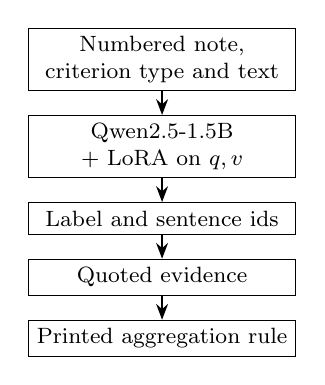
\begin{tikzpicture}[
  font=\footnotesize,
  box/.style={draw, align=center, inner sep=3pt, minimum width=34mm},
  arr/.style={-{Stealth[length=2mm]}, thick}
]
\node[box] (in) {Numbered note,\\criterion type and text};
\node[box, below=3mm of in] (model) {Qwen2.5-1.5B\\+ LoRA on $q,v$};
\node[box, below=3mm of model] (json) {Label and sentence ids};
\node[box, below=3mm of json] (quote) {Quoted evidence};
\node[box, below=3mm of quote] (agg) {Printed aggregation rule};
\draw[arr] (in) -- (model);
\draw[arr] (model) -- (json);
\draw[arr] (json) -- (quote);
\draw[arr] (quote) -- (agg);
\end{tikzpicture}
\caption{Screening path. The model emits a label and sentence ids. The application quotes those ids and aggregates criterion labels with a printed rule. The aggregation is not an expert trial label.}
\label{fig:workflow}
\end{figure}

The target is \texttt{Qwen/Qwen2.5-1.5B-Instruct}.
The model card used here is the one shipped with the weights \cite{qwen2025}.
It is a causal Transformer with 1.54\,B parameters (1.31\,B excluding embeddings), 28 layers, hidden size 1{,}536, 12 query heads and 2 key-value heads, SwiGLU intermediate size 8{,}960, RoPE, tied embeddings, and a 151{,}936-token Qwen2 tokenizer.
The context length is 32{,}768 tokens.
The license is Apache 2.0.
The bf16 file is 2.9\,GB.
The draft is \texttt{Qwen/Qwen2.5-0.5B-Instruct}, 0.49\,B parameters, the same tokenizer family, and the same chat template.

LoRA uses rank 8, alpha 16, dropout 0.05, and the \texttt{q\_proj} and \texttt{v\_proj} modules only.
Training uses batch size 1, gradient accumulation 8, AdamW at $2\times10^{-4}$, a linear schedule with 3\% warmup, gradient clipping at 1, bf16 on Metal, and gradient checkpointing.
The seed is 42.
Three epochs are run.
The checkpoint with the higher validation macro-F1 is kept, and training stops after two epochs without an improvement.
If a length does not fit, the script retries 768 and then 512.
Decoding for every graded number is greedy.
Sampling is not used.

\subsection{Metrics}
Accuracy and macro-F1 are reported over the six labels.
A class with no support and no predictions is left out of the macro average.
Per-class precision, recall, and F1, and a confusion matrix, are reported overall and again for inclusion and for exclusion.
An output that is not the required JSON is the class \texttt{<unparsed>}.

Evidence is scored as sets of sentence ids.
If both sets are empty, precision and recall are 1.
If the prediction is empty and the gold set is not, both are 0.
If the gold set is empty and the prediction is not, both are 0.
Otherwise precision is the size of the intersection divided by the size of the prediction, and recall divides by the size of the gold set.
Example-level macro scores average those example scores.
Micro scores pool the sentence occurrences.
The same scores are split by inclusion and exclusion.

The application also prints a trial-level line.
It is ineligible if any inclusion criterion is ``not included'' or any exclusion criterion is ``excluded''.
Otherwise it needs more information if any scored criterion is ``not enough information''.
Otherwise it is potentially eligible.
``Not applicable'' does not count.
This line is not a ground-truth label.

\subsection{Key-value cache}
The graded decoder does not call \texttt{generate}.
The uncached loop sends the full prefix at every step with \texttt{use\_cache=False}.
The cached loop prefills the prompt, stores each layer's keys and values, and then feeds one new token with \texttt{position\_ids} equal to the absolute length.
The first new token is produced by the prefill.
Later tokens are the decode loop.
Equality is the requirement: the two loops must emit the same greedy tokens.
The graded lengths are prompt/new pairs $(32,16)$, $(128,32)$, and $(512,64)$.
Timing uses a warmup and \texttt{torch.mps.synchronize()}.
End-of-sequence stopping is disabled in that benchmark so both loops emit the requested count.

\subsection{Tiled attention}
The reference module scales the scores by $1/\sqrt{d}$, adds a causal mask of $-\infty$, applies softmax, and multiplies by $V$.
The tiled module walks key blocks and keeps the online-softmax state: a running row maximum $m$, a running normalizer $\ell$, and a running unnormalized output.
A block whose scores are all $-\infty$ is skipped so that $\exp(-\infty-(-\infty))$ does not become NaN.
Neither module calls a fused scaled-dot-product kernel.
Both run in fp32.
The benchmark states that the Python tile is not expected to be faster.

\subsection{Speculative decoding}
The draft is the 0.5\,B base model.
The target is the 1.5\,B model with the adapter when the adapter exists.
Lookahead $\gamma$ starts at 4.
The draft proposes up to $\gamma$ greedy tokens.
One target forward verifies them.
The matching prefix is accepted.
On a mismatch, the target's token is kept and both caches are cropped to that point.
If the whole draft is accepted, the target's bonus token is appended.
The correctness test is token equality with the target's ordinary greedy output.
A slowdown is reported as a slowdown. It still meets the measurement requirement if the tokens match.

\section{Setup}
The machine is a MacBook Air with an Apple M5, 10 CPU cores, 8 GPU cores, and 16\,GB of unified memory.
Docker cannot use the GPU, so the application is a native FastAPI process and a Vite process.
PyTorch uses the Metal backend.
The base weights are downloaded into \texttt{models/} and are not committed.
The selected adapter is \texttt{outputs/task1/adapter}, and that folder is in the repository.
The epoch checkpoints stay local.
Commands, the seed, and the metric definitions are in the README and in \texttt{configs/train.json}.

\section{Results}
\label{sec:results}
Figure~\ref{fig:curve} shows the training loss and the validation macro-F1 used to pick the checkpoint.
The selected epoch is 1, with validation macro-F1 0.458 during training.
0 train rows lost an expert sentence id to truncation at the trained length.
The 601 teaching annotations were repeated only inside the train split, up to the majority count of each criterion type and at most eight times, which produced 1190 encoded rows.

\begin{figure}[t]
\centering
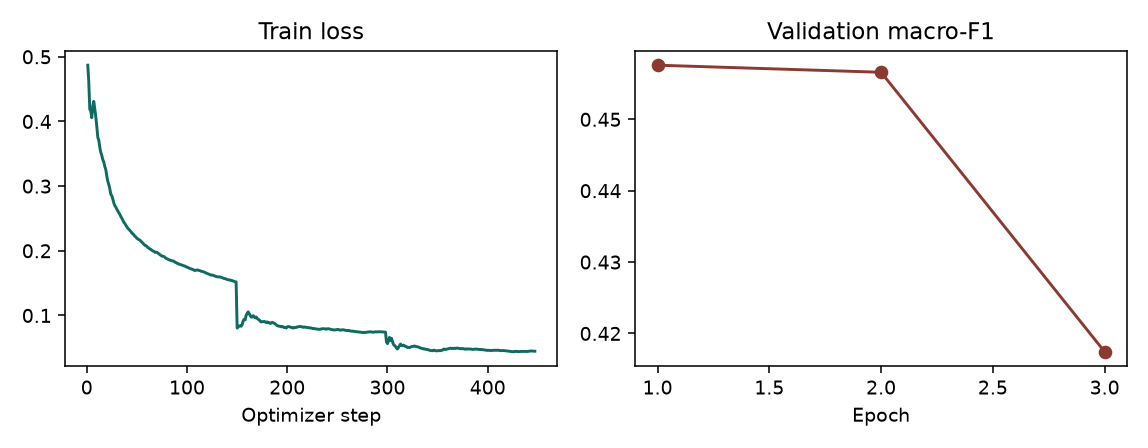
\includegraphics[width=0.95\linewidth]{../results/task1/training_curve.png}
\caption{Train loss by optimizer step and validation macro-F1 by epoch. The checkpoint with the higher validation macro-F1 is the one that is evaluated.}
\label{fig:curve}
\end{figure}

Table~\ref{tab:compare} compares the untouched base model and the adapter on the same rows and the same greedy decoder.
On validation, accuracy moves from 9.2\% to 67.5\% and macro-F1 moves from 0.108 to 0.458.
On the held-out test set, which was scored once, accuracy is 10.7\% for the base model and 67.5\% for the adapter.
Test macro-F1 is 0.150 and 0.492.
Example-level evidence F1 on the test set is 0.214 and 0.724.

\begin{table}[t]
\centering
\caption{Base model and adapter. Decoding is greedy. The test split was scored once.}
\label{tab:compare}
\begin{tabular}{lcccc}
\toprule
Split & Model & Accuracy & Macro-F1 & Evidence F1 \\
\midrule
Validation & Base & 9.2\% & 0.108 & 0.164 \\
Validation & Adapter & 67.5\% & 0.458 & 0.646 \\
Test & Base & 10.7\% & 0.150 & 0.214 \\
Test & Adapter & 67.5\% & 0.492 & 0.724 \\
\bottomrule
\end{tabular}
\end{table}

Table~\ref{tab:perclass} is the adapter's per-class precision, recall, and F1 on the test set.
Rare labels stay rare: a high accuracy can still hide a weak F1 on ``excluded'' or ``not included''.
Figure~\ref{fig:cm} is the adapter's test confusion matrix.
The inclusion and exclusion matrices are saved beside it and are not a collapsed yes/no task.

\begin{table}[t]
\centering
\caption{Adapter, test set, per-class scores. Support is the number of expert labels.}
\label{tab:perclass}
\begin{tabular}{lcccc}
\toprule
Label & Support & Precision & Recall & F1 \\
\midrule
included & 27 & 0.880 & 0.815 & 0.846 \\
not included & 7 & 0.238 & 0.714 & 0.357 \\
excluded & 0 & 0.000 & 0.000 & 0.000 \\
not excluded & 91 & 0.730 & 0.923 & 0.816 \\
not enough information & 66 & 0.769 & 0.303 & 0.435 \\
not applicable & 15 & 0.471 & 0.533 & 0.500 \\
\bottomrule
\end{tabular}
\end{table}

\begin{figure}[t]
\centering
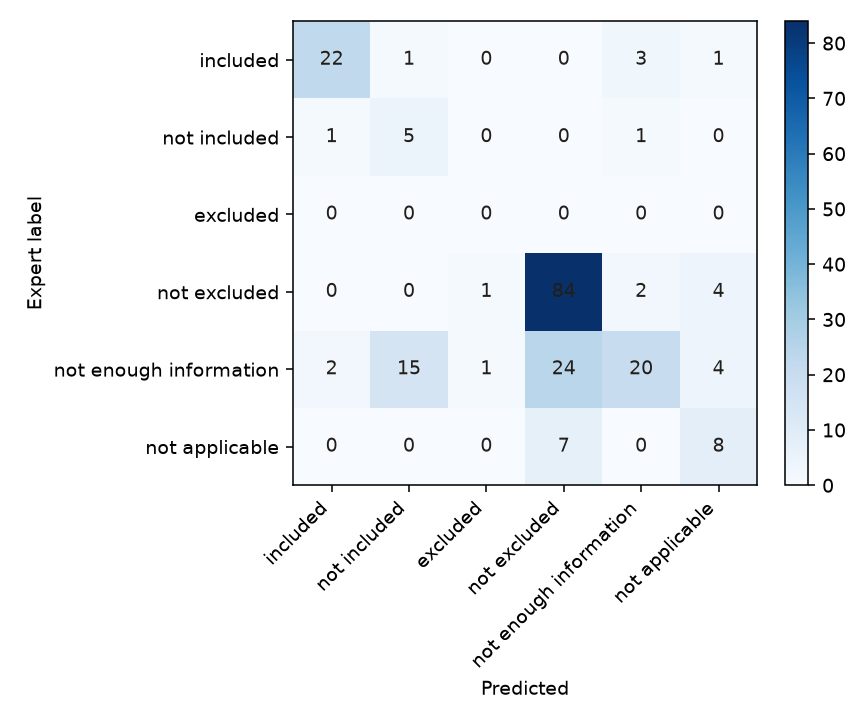
\includegraphics[width=0.72\linewidth]{../results/task2/confusion_test_adapter_overall.png}
\caption{Confusion matrix for the adapter on the test set. Rows are expert labels and columns are predictions. Unparsed outputs are their own column.}
\label{fig:cm}
\end{figure}

Table~\ref{tab:evidence} applies the empty-set rule to the adapter on the test set.
Both-empty counts as a match. A citation where the expert cited nothing scores zero, and so does a missing citation where the expert cited something.

\begin{table}[t]
\centering
\caption{Adapter evidence scores on the test set. Macro is the mean of the example scores. Micro pools sentence occurrences.}
\label{tab:evidence}
\resizebox{\columnwidth}{!}{%
\begin{tabular}{lcccccc}
\toprule
Slice & P & R & F1 & Micro P & Micro R & Micro F1 \\
\midrule
Overall & 0.719 & 0.743 & 0.724 & 0.380 & 0.660 & 0.482 \\
Inclusion & 0.567 & 0.613 & 0.574 & 0.407 & 0.742 & 0.526 \\
Exclusion & 0.805 & 0.818 & 0.809 & 0.320 & 0.500 & 0.390 \\
\bottomrule
\end{tabular}}
\end{table}

The base model left 0 test outputs unparsed.
The adapter left 0 unparsed and cited an id outside the note on 0 rows.
Table~\ref{tab:errors} lists the reviewed failures. Each row in the accompanying \texttt{errors.md} stores the criterion, the expert label, the prediction, the quoted sentences, and why it failed.

\begin{table}[t]
\centering
\caption{Reviewed test failures for the adapter. The full quotations are in \texttt{results/task2/errors.md}.}
\label{tab:errors}
\resizebox{\columnwidth}{!}{%
\begin{tabular}{llccc}
\toprule
Category & Id & Type & Expert & Predicted \\
\midrule
wrong\ label & 164 & inclusion & not included & included \\
missing\ information & 169 & exclusion & not enough information & not excluded \\
missed\ gold\ sentence & 185 & inclusion & included & not enough information \\
empty\ gold\ but\ model\ cited & 161 & inclusion & not included & not included \\
not\ applicable\ confusion & 683 & exclusion & not applicable & not excluded \\
additional\ mismatch & 162 & inclusion & not included & not included \\
additional\ mismatch & 163 & inclusion & not included & not included \\
additional\ mismatch & 166 & exclusion & not excluded & not excluded \\
truncation\ would\ drop\ gold & 160 & inclusion & included & included \\
\bottomrule
\end{tabular}}
\end{table}

Table~\ref{tab:kv} checks the hand-written cache against the uncached loop on the adapter model.
Tokens match on 2 of 3 graded lengths. At 32/16 the first disagreement is index 42: the cache emits token 19 and the uncached loop emits token 20. A fresh one-step cache on that shared prefix agrees with the full forward. The top logits differ by one bf16 unit, so the long-running cache breaks a tie. The position ids and the mask are the same on both paths.
Prefill is timed separately from the later tokens.
The first new token is produced by the prefill, so the decode rate does not include it in the same way the speculative rate does.
The uncached loop resends the whole prefix, which is why its decode time grows with the prompt length.

\begin{table*}[t]
\centering
\caption{Cached and uncached greedy decoding. EOS is disabled. Times are seconds after one warmup. Memory is peak megabytes.}
\label{tab:kv}
\begin{tabular}{lcccccccc}
\toprule
Length & Equal & Prefill & Dec. cache & Dec. plain & Tok/s c. & Tok/s p. & MB c. & MB p. \\
\midrule
32/16 & false & 0.053 & 0.535 & 0.949 & 29.9 & 16.9 & 3161 & 3161 \\
128/32 & true & 0.098 & 1.033 & 4.527 & 31.0 & 7.1 & 3170 & 4194 \\
512/64 & true & 0.289 & 2.174 & 23.769 & 29.6 & 2.7 & 4218 & 4186 \\
\bottomrule
\end{tabular}
\end{table*}

Table~\ref{tab:attn} compares reference attention with tiled online softmax in fp32.
The largest absolute error in these cases is 5.96e-07.
The tiled loop is slower. That is the expected result for a Python block loop against a single matrix softmax, and it is not a fused kernel.

\begin{table}[t]
\centering
\caption{Reference and tiled attention. Shapes are batch, heads, sequence, and head size. Times are seconds.}
\label{tab:attn}
\resizebox{\columnwidth}{!}{%
\begin{tabular}{lcccccc}
\toprule
Shape & Block & Causal & Max abs & Mean abs & Ref. & Tiled \\
\midrule
1,1,8,16 & 4 & true & 1.19e-07 & 2.37e-08 & 0.00004 & 0.00006 \\
2,4,17,32 & 8 & true & 5.96e-07 & 4.45e-08 & 0.00005 & 0.00013 \\
1,2,64,64 & 16 & true & 3.58e-07 & 2.73e-08 & 0.00005 & 0.00019 \\
1,2,64,64 & 16 & false & 4.77e-07 & 2.57e-08 & 0.00003 & 0.00017 \\
1,4,128,64 & 32 & true & 4.77e-07 & 2.71e-08 & 0.00014 & 0.00042 \\
\bottomrule
\end{tabular}}
\end{table}

Table~\ref{tab:spec} is greedy speculative decoding with lookahead 4.
The draft is the 0.5\,B base model and the target is the adapter 1.5\,B model.
3 of 4 prompts matched the target's ordinary greedy tokens.
On the prompt that differs, the full-forward top two logits also differ by one bf16 unit, and the speculative token is that forward's argmax.
Acceptance rate is the fraction of drafted tokens that were kept.
A speedup below 1 is a slowdown. The token match is the correctness result.

\begin{table}[t]
\centering
\caption{Speculative decoding against target greedy decoding. 32 new tokens, lookahead 4.}
\label{tab:spec}
\resizebox{\columnwidth}{!}{%
\begin{tabular}{lcccccc}
\toprule
Prompt & Equal & Accept & Greedy tok/s & Spec. tok/s & Speedup & Peak MB \\
\midrule
1 & true & 0.622 & 20.8 & 13.8 & 0.663 & 4193 \\
2 & false & 0.447 & 16.5 & 9.7 & 0.589 & 4201 \\
3 & true & 0.667 & 24.8 & 20.4 & 0.823 & 4193 \\
4 & true & 0.622 & 23.6 & 17.0 & 0.721 & 4193 \\
\bottomrule
\end{tabular}}
\end{table}


\subsection{Application}
Figure~\ref{fig:app} is the browser after a three-sentence note, one inclusion criterion, and one exclusion criterion.
The notice at the top says this is not an enrollment decision.
Each card shows the label, whether information is missing, and the quoted sentence.
The overall line is potentially eligible, and the text beside it is the aggregation rule.
Figure~\ref{fig:error} is the same page after the note was cleared and screening was started again.
The empty note is rejected, and the previous cards remain, including the download button.
Figure~\ref{fig:lab} is the inference lab after the tiled-attention button.
The maximum absolute error on that click is $7.15\times10^{-7}$, and the tiled loop is slower than the reference.
Those numbers were produced by the button. They are not a stored chart.

\begin{figure}[t]
\centering
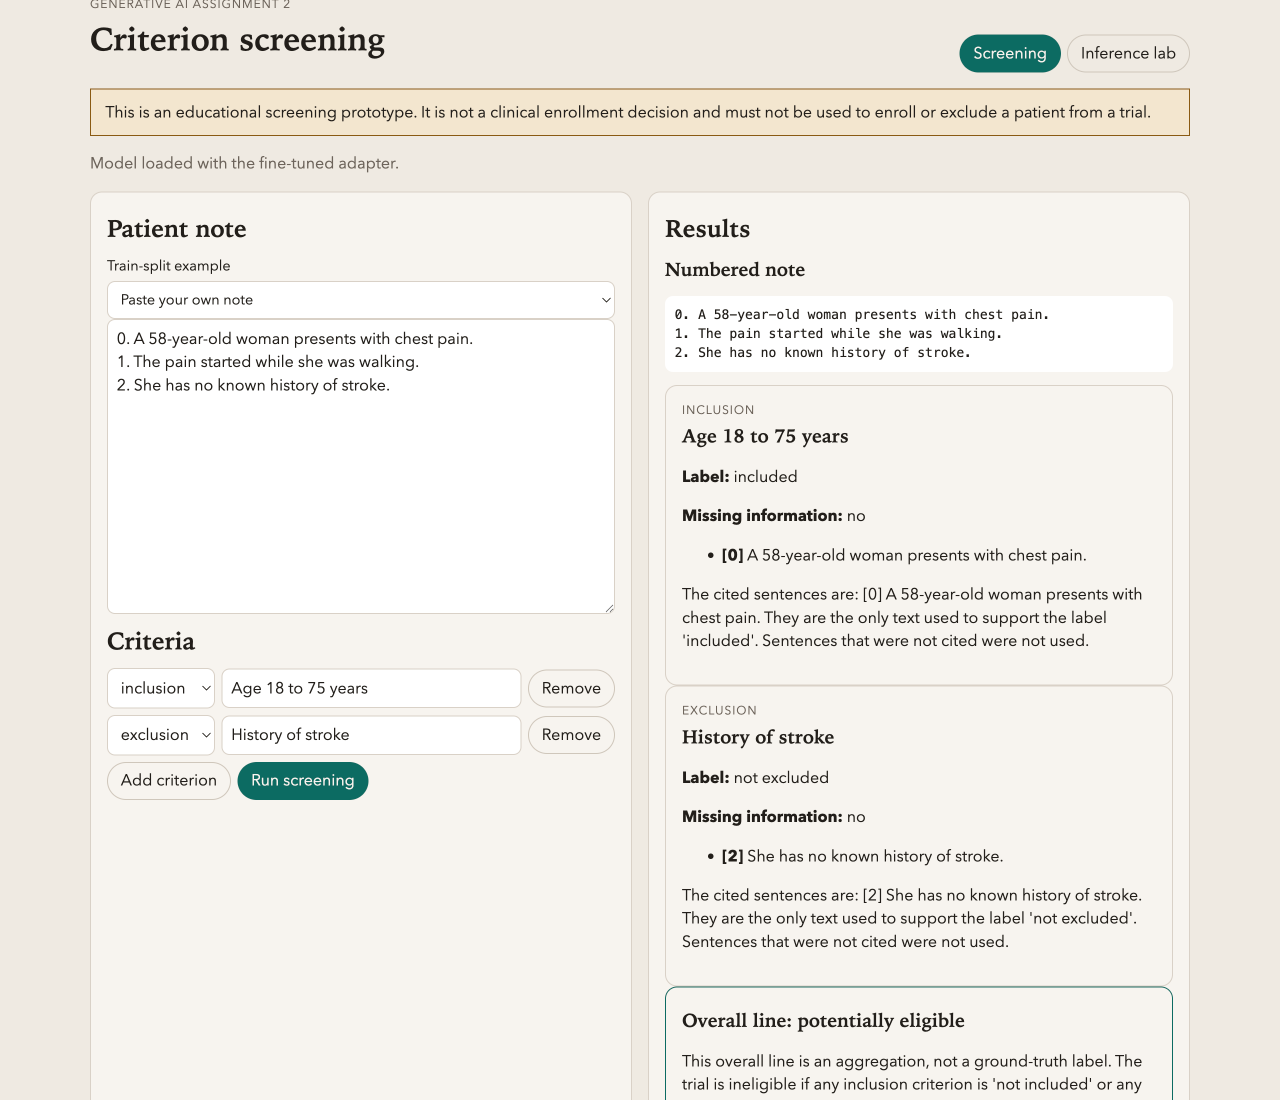
\includegraphics[width=\linewidth]{figures/screen.png}
\caption{Screening page. The notice, the label, the quoted sentence, and the start of the aggregation line are visible together.}
\label{fig:app}
\end{figure}

\begin{figure}[t]
\centering
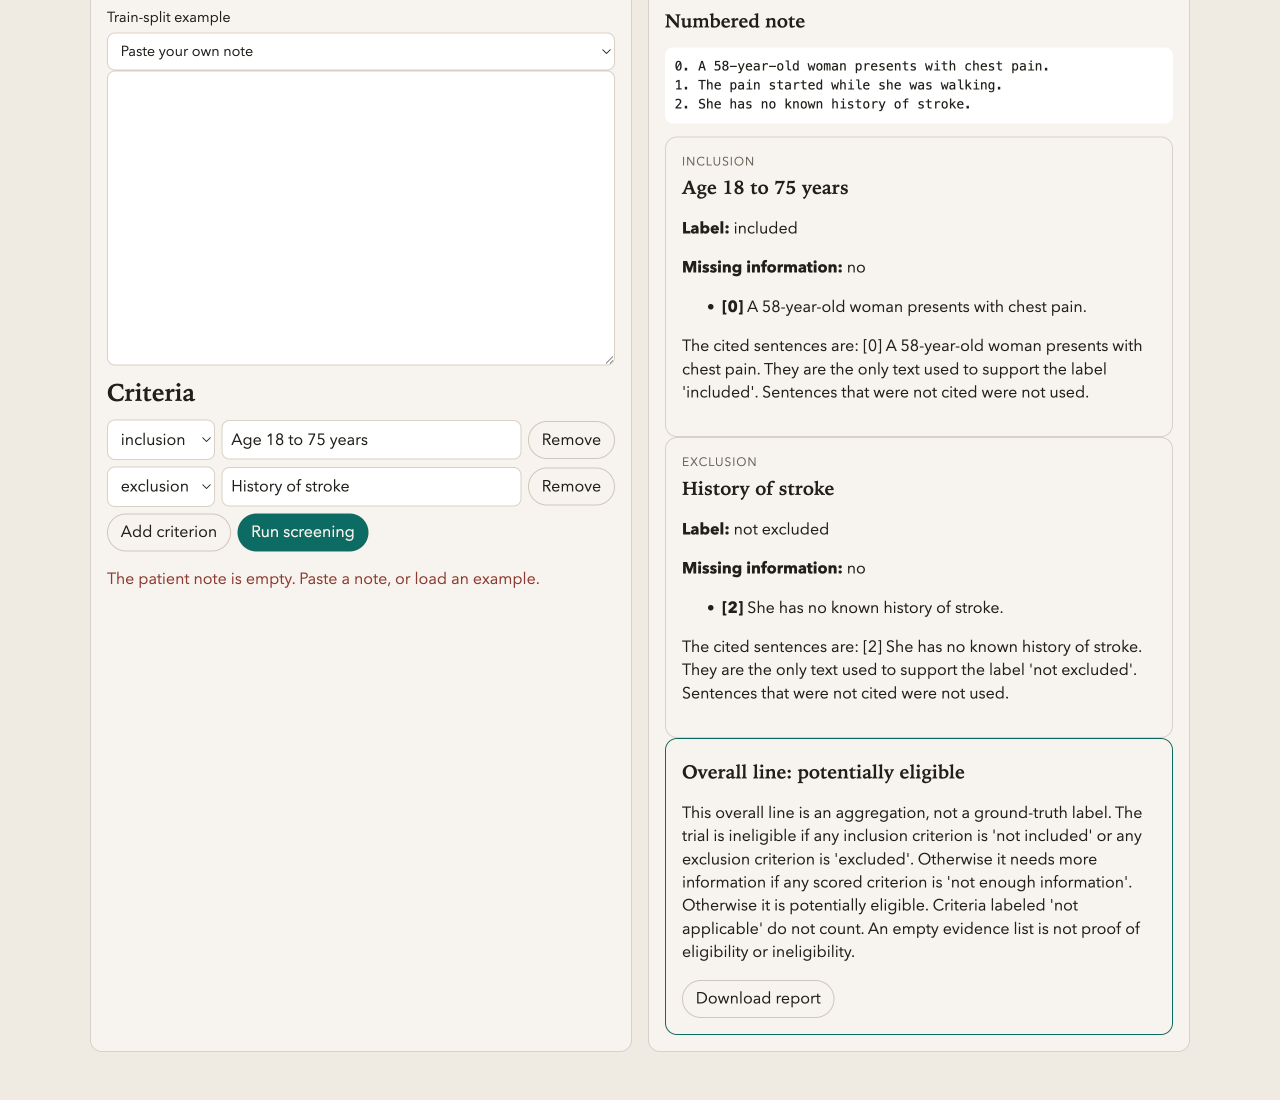
\includegraphics[width=\linewidth]{figures/error.png}
\caption{An empty note is rejected. The previous criterion cards and the aggregation line stay on the page.}
\label{fig:error}
\end{figure}

\begin{figure}[t]
\centering
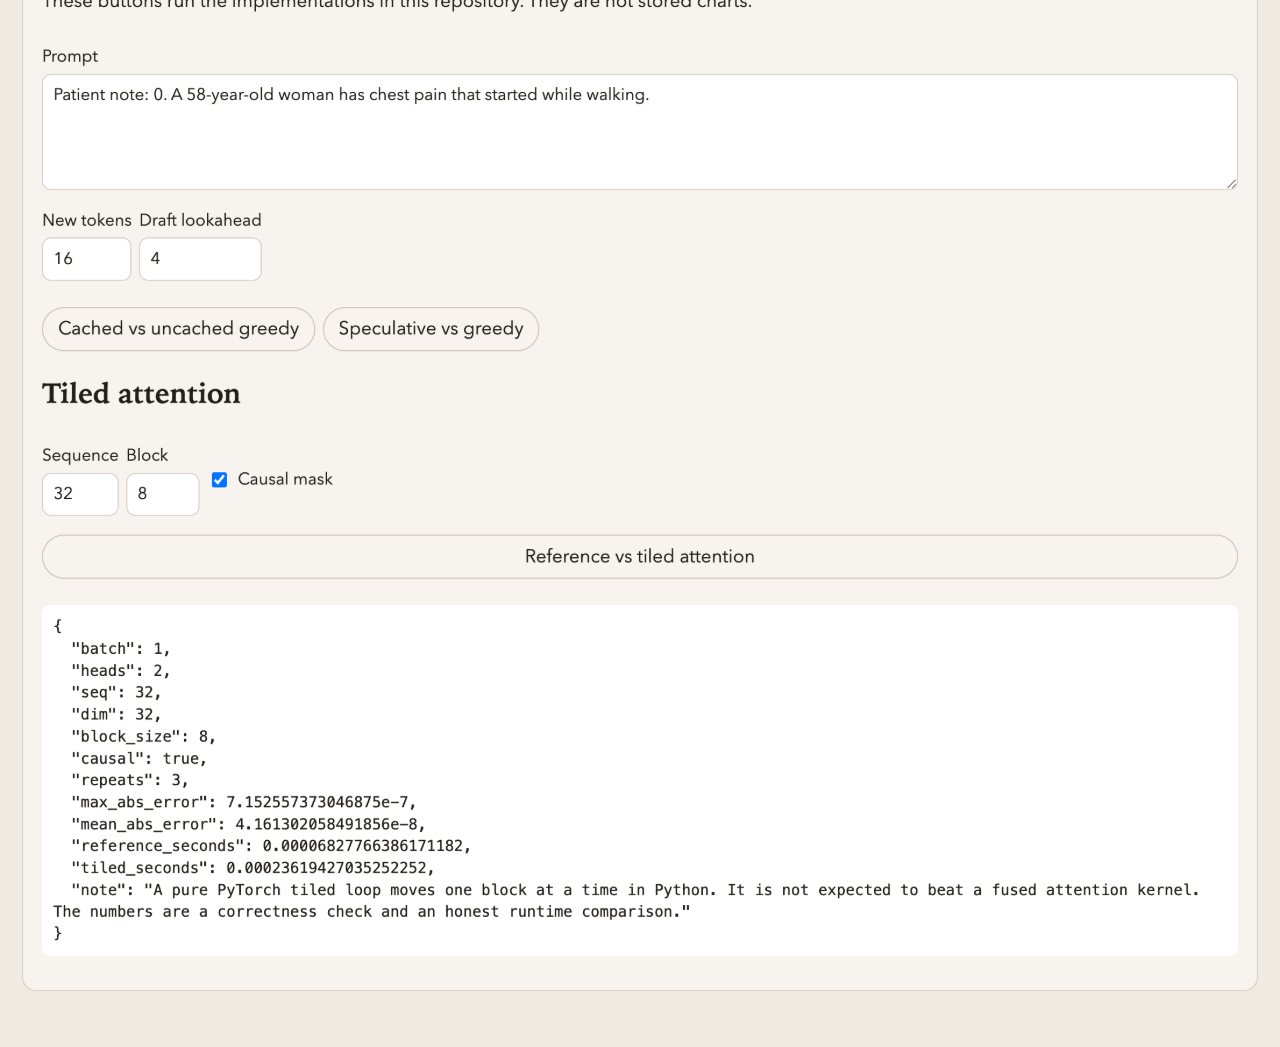
\includegraphics[width=\linewidth]{figures/lab.png}
\caption{Inference lab after one tiled-attention run. The result includes the maximum error and both runtimes.}
\label{fig:lab}
\end{figure}

\section{Limitations}
The machine has 16\,GB of unified memory, so the target is a 1.54\,B model and the context used for training is at most 1{,}024 tokens.
The notes in this release happen to fit, but a longer clinical note would lose sentences from the end, and a gold id in that tail would be unlearnable.
The label set is severely unbalanced. ``Excluded'' has 10 rows in the whole release, and ``not included'' has 23.
Macro-F1 on those classes is a hard target for a model this small, and oversampling does not create new evidence.
The trial-level sentence in the application is an aggregation of criterion labels.
It is not an expert trial decision, and the screen says so.
Empty citations are not treated as eligibility.
The system is an educational prototype. It must not be used to enroll or exclude a patient.

\section{Conclusion}
A 1.54\,B decoder can be adapted, on a 16\,GB laptop, to emit criterion labels and sentence ids for the TrialGPT annotations without collapsing the six labels and without training on the released GPT-4 fields.
The hand-written cache matches uncached greedy decoding at prompt lengths 128 and 512. At prompt length 32 the paths differ by one token where the bf16 logits are tied. The tiled online softmax matches the reference attention within floating-point error. Greedy speculative decoding matches the target on three of four prompts, and the miss is the same kind of one-unit tie.
The browser screen quotes the cited sentences, flags missing information, and applies an aggregation rule that is printed next to the result.
The held-out numbers measure that small model. They do not replace an expert.

\section*{Acknowledgment}
An AI coding assistant (Cursor, with a large language model) helped implement the software and draft this paper.
The author remains responsible for the split, the metrics, the decoding code, and the numbers taken from the saved logs.

\begin{thebibliography}{00}
\bibitem{vaswani2017attention}
A. Vaswani, N. Shazeer, N. Parmar, J. Uszkoreit, L. Jones, A. N. Gomez, L. Kaiser, and I. Polosukhin,
``Attention is all you need,'' in \emph{Advances in Neural Information Processing Systems}, 2017.

\bibitem{hu2022lora}
E. J. Hu, Y. Shen, P. Wallis, Z. Allen-Zhu, Y. Li, S. Wang, L. Wang, and W. Chen,
``LoRA: Low-rank adaptation of large language models,'' in \emph{Proc. ICLR}, 2022.

\bibitem{milakov2018online}
M. Milakov and N. Gimelshein,
``Online normalizer calculation for softmax,'' arXiv:1805.02867, 2018.

\bibitem{dao2022flashattention}
T. Dao, D. Y. Fu, S. Ermon, A. Rudra, and C. R\'e,
``FlashAttention: Fast and memory-efficient exact attention with IO-awareness,'' in \emph{Advances in Neural Information Processing Systems}, 2022.

\bibitem{leviathan2023speculative}
Y. Leviathan, M. Kalman, and Y. Matias,
``Fast inference from transformers via speculative decoding,'' in \emph{Proc. ICML}, 2023.

\bibitem{jin2024trialgpt}
Q. Jin, Z. Wang, C. S. Floudas, F. Chen, C. Gong, D. Bracken-Clarke, E. Xue, Y. Yang, J. Sun, and Z. Lu,
``Matching patients to clinical trials with large language models,'' \emph{Nature Communications}, vol. 15, p. 9074, 2024.

\bibitem{qwen2025}
Qwen Team,
``Qwen2.5 technical report,'' arXiv:2412.15115, 2025.
\end{thebibliography}

\end{document}
